%
% Layout retirado de http://www.di.uminho.pt/~prh/curplc09.html#notas
%
\documentclass{report}
\usepackage[portuges]{babel}
\usepackage[utf8]{inputenc}
\usepackage[latin1]{inputenc}
\usepackage{graphicx}

\usepackage{url}
\usepackage{enumerate}

%\usepackage{alltt}
%\usepackage{fancyvrb}
\usepackage{listings}
%LISTING - GENERAL
\lstset{
	basicstyle=\small,
	numbers=left,
	numberstyle=\tiny,
	numbersep=5pt,
	breaklines=true,
    frame=tB,
	mathescape=true,
	escapeinside={(*@}{@*)}
}

\usepackage{xspace}

\parindent=0pt
\parskip=2pt

\setlength{\oddsidemargin}{-1cm}
\setlength{\textwidth}{18cm}
\setlength{\headsep}{-1cm}
\setlength{\textheight}{23cm}

\def\darius{\textsf{Darius}\xspace}
\def\antlr{\texttt{AnTLR}\xspace}
\def\pe{\emph{Publicação Eletrónica}\xspace}

\def\titulo#1{\section{#1}}
\def\supers#1{{\em Supervisores: #1}\\ }
\def\area#1{{\em \'{A}rea: #1}\\[0.2cm]}
\def\resumo{\underline{Resumo}:\\ }


%%%%\input{LPgeneralDefintions}

\title{Projeto (3º ano de LCC)\\ \textbf{VMS, Simular Visual para a máquina de Stack Virtual VM}\\ Relatório de Desenvolvimento}
\author{Adriano Campinho\\ (a79032) \and Vasco Leitão\\ (a79220) }
\date{\today}

\begin{document}

\maketitle
\begin{abstract}
	\quad Este documento apresenta o relatório desenvolvido no âmbito da Unidade Curricular de Projecto, pretendendo
	explicitar o processo de conceção e implementação do mesmo, assim como as escolhas tomadas e as pretendidas resoluções
	para cada problema exposto no enunciado fornecido, prestando especial atenção ao modo de utilização do simulador; \\
	\\
	\\
	\\
  \\
	\supers{Pedro Rangel Henriques e José João}
	\area{Processamento de Linguagens}

\end{abstract}

\tableofcontents

\chapter{Introdução} \label{intro}

\quad Nos últimos anos, temos usado nas disciplinas de Processamento de Linguagens (e
Compiladores) a máquina virtual VM, uma máquina de stack que suporta inteiros, reais e
strings e tem uma heap para permitir um uso dinâmico da memória (necessário por exemplo
para implementar listas ligadas). A VM é programada em Assembly e que disponibiliza um
conjunto de instruções máquina mínimo e muito compreensível, o que a torna
pedagogicamente muito relevante como máquina objeto (destino) em tarefas de compilação.
\\
\\
\null\quad Para que o uso da VM seja realmente um bom instrumento de trabalho nestes cursos, é
fundamental que exista um simulador que permita testar (de preferência passo a passo) o
código gerado. Atualmente existe, como é de conhecimento de todos, um Assembler para
traduzir o Assembly produzido numa lista de códigos máquina e existe um interpretado que
executa esse código e que fornece uma interface visual que permite acompanhar a execução
verificando a evolução dos vários blocos de memória e dos registo de controlo da máquina.
\\
\\
\null\quad Esta versão, codificada em Java, está funcional e pode ser usada, mas tem alguns problemas de
implementação, nomeadamente o elevado tempo de execução, quando os programas
aumentam um pouco.
\\
\\
\null\quad Neste projeto pretende-se que os alunos reconstruam o simulador com interface interativo e
visual para a máquina VM desde o início, em Java ou em C (conforme preferência do grupo)
produzindo um executável que evite os problemas atuais.

\chapter{Análise e Especificação} \label{ae}
\section{Descrição Informal da Máquina}

\quad Trata-se duma máquina de pilhas (por oposição às máquinas de registos), esta e composta duma pilha de execução, duma pilha de chamadas,
duma zona de código e de duas heaps:

\begin{center}
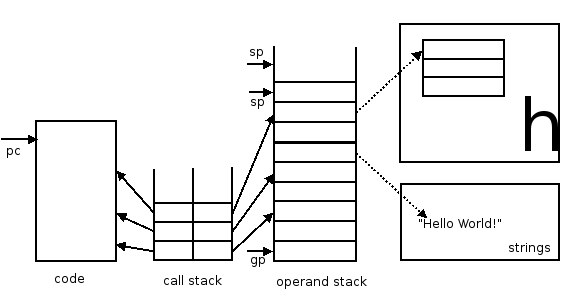
\includegraphics{stacks.png}
\end{center}

\paragraph{\quad Code -}
Esta pilha contem o conjunto das instruções do programa, esta e preenchida no inicio da execução do programa, mantendo-se igual
do princípio ao fim da execução do mesmo;
\paragraph{\quad Operation Stack -}
Esta pilha contem valores guardados no registo da maquina, estes são todos indexados, podendo ser do tipo inteiro, real e endereço;
\paragraph{\quad Heap -}
Esta pilha contem cadeias de caracteres (strings), cada uma destas referenciado por endereços, cada bloco,
contendo um certo numero de caracteres;
\paragraph{\quad Call Stack -}
Esta pilha contem blocos estruturados, cada um destes referenciado por endereços, cada bloco
estruturado contem um certo numero de valores (estes são do mesmo tipo dos que se podem encontrar na Operation Stack);
\\
\\
\null\quad Um endereço pode apontar para quatro tipos de informação: para código, para a
pilha, para um bloco estruturado ou para uma string.
Ao longo da execução do programa são guardados os seguintes quatro registos:
\begin{itemize}
	\item \textit{\textbf{SP}} (Stack Pointer) o registo aponta para o topo corrente da pilha/ para a primeira célula livre da pilha.
	\item \textit{\textbf{FP}} (Frame Pointer) o registo aponta para o endereço de base das variáveis locais.
	\item \textit{\textbf{GP}} (Global Pointer) o registo contem o endereço de base das variáveis globais.
	\item \textit{\textbf{PC}} (Program Counter) o registo aponta para a instrução corrente (da zona de código) por executar.
\end{itemize}

A pilha de chamada permite guardar as chamadas: contém pares de apontadores
(i, f). O endereço i guarda o registo de instrução pc e f o registo fp.

\subsubsection{Instruções}

\quad As instruções são designadas por um nome e podem aceitar um ou dois parâmetros.
Estes parâmetros podem ser dos seguintes tipos:
\begin{itemize}
\item Constantes inteiras,
\item Constantes reais,
\item Cadeias de caracteres delimitadas por aspas. Estas cadeias de caracteres seguem as
mesmas regras de formatação que as cadeias da linguagem C (em particular no que
diz respeito aos caracteres especiais como \", \n ou \textbackslash\textbackslash ),
\item Uma etiqueta simbólica designando uma zona no código.
\end{itemize}

\quad O conjunto das instruções pode ser encontrado no documento original fornecido com as fontes da maquina virtual aqui descrita,
destas foram ignoradas as primitivas gráficas, não sendo esta uma implementação de uma versão gráfica da maquina virtual;

\section{Planeamento e objetivos}
\quad O simulador deve ser implementado de forma a funcionar num maior numero de ambientes possível:
deve ser possível correr a simulação de vários modos possibilitando uma simulação interativa de cada programa.
Existindo a possibilidade do jogador interagir com a simulação através da linha de comandos ou através de uma Interface
gráfica a ser desenvolvida.\\
\null\quad Podemos então dividir o projecto em 3 grandes grupos:
\begin{itemize}
	\item \textbf{Parser:} um parser que receba o input
	(programas a ser simulados) partindo-os em partes para que possam ser geridas por um outro grupo,
	verificando se o ficheiro esta no formato correto, caso contrario apontando onde estarão os possíveis problemas;

	\item \textbf{Simulador:} um programa que através do input recebido do parser e, se necessário, do input do utilizador,
	faca a simulação em si do programa;

	\item \textbf{Interface Gráfica:} uma interface que permita ao utilizador interagir com a execução do simulador,
	e dando-lhe acesso a informação sobre o estado atual da maquina;
	Cada vez que o utilizador interatue com a interface (e.g. clicando num botão), esta deve ser atualizada,
	refletindo as alterações feitas no estado na maquina e na interface.
\end{itemize}

\section{Especificação do Requisitos}
\quad Esta secção de forma mais especifica os requisitos de cada um dos grupos de desenvolvimento demonstrando os problemas que
surgiram durante cada fase:

\subsection{Parser}

\quad O parser deve aceitar programas com a seguinte sintaxe:

\begin{center}
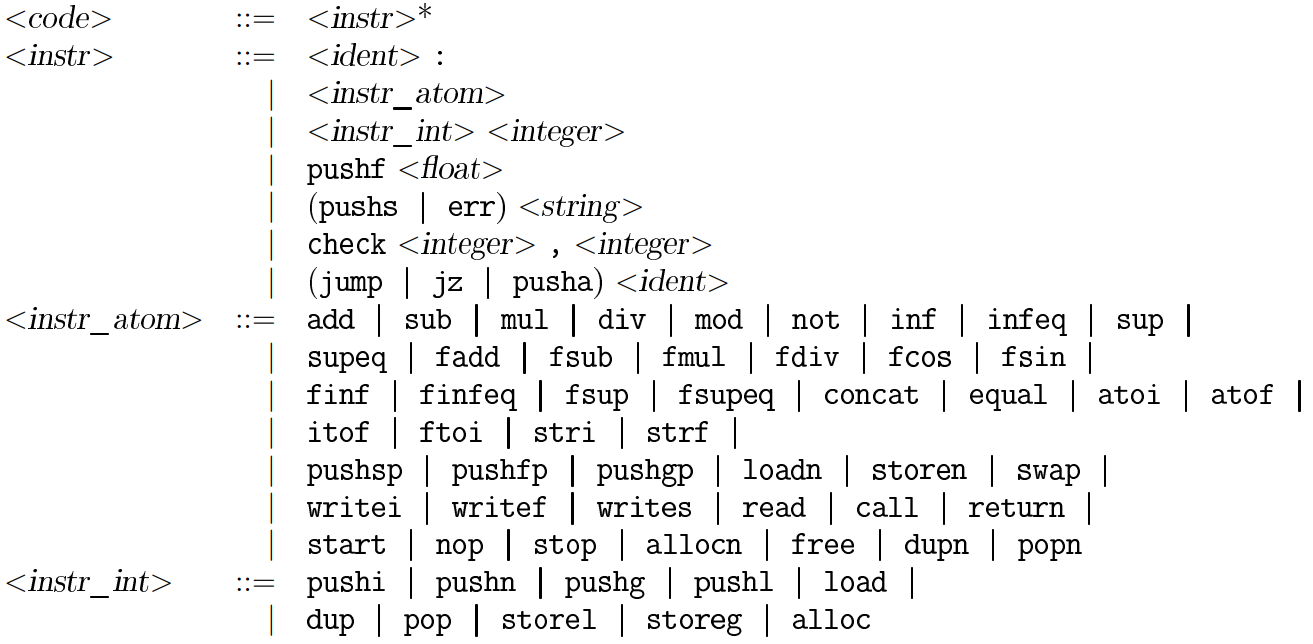
\includegraphics[width=\textwidth]{sintaxe.png}
\end{center}

\quad Ainda, o parser devera ignorar tudo o que sirva para embelezar o código do programa (sejam espaços a mais, linhas em branco etc.),
assim como devera ser possível a utilização de comentários que deverão ser ignorados pelo mesmo.

\subsection{Processador}

\quad O processador devera receber o programa tratado pelo Parser e executar as instruções produzindo o resultado
esperado (descrito no documento referido acima), permitindo ao utilizador controlar a execução do programa;

\subsection{Interface Gráfica}
\quad A interface deve permitir ao utilizador executar as seguintes ações:
\begin{itemize}
\item Realizar 1 passo na execução do programa;
\item Realizar n passos (passado como argumento) na execução do programa;
\item Realizar a execução do programa ate ao fim de uma vez só;
\item Carregar um programa para ser simulado;
\item Recarregar o programa que esta atualmente a ser simulado;
\item Em qualquer momento da execução do programa, mostrar o estado actual da maquina (stacks e pointers);
\item Permitir ao utilizador introduzir input para o programa quando necessário;
\item Permitir ao utilizador introduzir múltiplas linhas de input de uma vez;
\item Carregar um ficheiro com o input para ser lido por um programa;
\end{itemize}

\chapter{Concepção/desenho da Resolução}
\section{Organização do código}

Em termos de organização do código, este foi dividido nos seguintes ficheiros:

\begin{itemize}
\item \textbf{check.sh*} - Coisas
\item \textbf{README} - Coisas
\item \textbf{structs/} - Coisas
\item \textbf{vmsMan.1} - Coisas
\item \textbf{inst\_err} - Coisas
\item \textbf{lex.l} - Coisas
\item \textbf{semantic.c} - Coisas
\item \textbf{syntax.y} - Coisas
\item \textbf{interface.c} - Coisas
\item \textbf{makefile} - Coisas
\item \textbf{semantic.h} - Coisas
\item \textbf{vms.c} - Coisas
\end{itemize}

\subsection{Estruturas}

Em termos de estruturas criadas, estas foram divididas nos seguintes grupos
(sendo que cada grupo representa um par de ficheiros .h e .c):


\begin{itemize}
	\item \textbf{array} - Coisas
	\item \textbf{callStack} - Coisas
	\item \textbf{code} - Coisas
	\item \textbf{heap} - Coisas
	\item \textbf{opStack} - Coisas
	\item \textbf{types} - Coisas
\end{itemize}
\section{Fases de Desenvolvimento}
\subsection{Parser}
\quad Falar flex etc.
\subsection{Processador}
\quad Estruturas de dados etc.
\subsection{Interface}
\quad Nao faco ideia

\chapter{Guia de Utilização e Testes}
\section{Modo de utilização}
\quad Esta máquina destina-se a uma utilização interactiva do utilizador, para visualizar a execução de um programa.\\
A execução poderá ser conduzida passo a passo, ou ser feita de uma só vez.\\
Sendo feita da seguinte forma:\\

\quad \textbf{vms [opção] ficheiro.vm} OU \textbf{vms opção [ficheiro.vm]}\\

O projeto desenvolvido, tem 3 opções de utilização, estas são:
\paragraph{\quad Máquina em Modo Silencioso (sem flag de opção)}
	O programa passado como argumento, e executado de inicio ao fim, apenas permitindo ao utilizador introduzir input quando pedido;
\paragraph{\quad Máquina em Modo Debug (-d)}
	O modo Debug permite ao utilizador o acesso a mais informação sobre o programa, disponibilizando
  os seguintes comandos, que permitem uma execução interativa do programa:
\begin{itemize}
	\item \textbf{run:} executa o programa ate ao fim;
	\item \textbf{next 'n':} executa 'n' passos;
	\item \textbf{file 'f':} "carrega" o ficheiro 'f' para ser executado;
	\item \textbf{reload:} recarrega o ficheiro no "local" do ultimo ficheiro executado;
	\item \textbf{quit:} termina a execução do simulador;
\end{itemize}
\paragraph{\quad Máquina em Modo Interface (-g)}
  O modo Interface
\section{Mensagens de erro}

\begin{itemize}
\item "Error: Index out of array"
\item "Error: fp == sp"
\item "Error: Opening file"
\item "Error: You must specify a '-d' or '-g' option, or a program file\nTry 'man vms' for more information.\n"
\item "Error: Invalid type ( write / not / equal / padd second arg not int / padd first argument not adress / alocn / free /
 atox arg is not heap adress / itof / ftoi / stri / strf / loadn / load / dupn / popn / pon / storen / jz / call )"
\end{itemize}

\section{Alternativas, Decisões e Problemas de Implementação}
\section{Testes realizados e Resultados}
Mostram-se a seguir alguns testes feitos (valores introduzidos) e
os respectivos resultados obtidos:

\chapter{Conclusão} \label{concl}
\quad Neste relatório descreveu-se o processo de conceção e implementação do projecto pedido pelo
enunciado, nomeadamente o parser, o simulador e a interface gráfica, alem de descrever em detalhe
o funcionamento da maquina referida.\\
\null\quad Apesar de estarmos satisfeitos com o trabalho desenvolvido, há ainda espaço para muitas
melhorias desta implementação. Enumeram-se algumas ideias que, por falta de tempo, não foram
(ainda) concretizadas:

\begin{itemize}
\item Criar um conjunto grande de ficheiros de testes, que sirvam tanto para provar/verificar a
implementação da maquina, assim como servir de exemplo da correcta instalação da mesma;
\item Fazer melhorias no espaçamento da interface gráfica, permitindo a utilização mais fácil em janelas mais pequenas;
\end{itemize}

\bibliographystyle{alpha}
\bibliography{relprojLayout}

\end{document}
